\subsection{Example}\label{sec:set-example}

TK - Introduce, 2D identity map, known observed (square in center with area 1/100, i.e. density value of 100).

\begin{python}
"""
Set up and solve problem with identity map
"""
# import libraries
import bet.sample as sample
import bet.sampling.basicSampling as bsam
import bet.calculateP.simpleFunP as simpleFunP
import bet.calculateP.calculateP as calculateP
import numpy as np
import scipy.stats as sstats
# define input space parameters and model to instantiate sampler object
dimension = 2
numSamples = 100
I = np.eye(dimension)
def model(input_samples):
        return (I@input_samples.T).T
sampler = bsam.sampler(model)
# instantiate objects that hold input/output samples
# default random sample set is uniform over unit domain (normalized space)
input_set = input_samples = bsam.random_sample_set('r',input_obj=dimension, num_samples=numSamples)
param_ref = np.array([0.5, 0.5])
input_set.set_reference_value(param_ref)
# Estimate volumes of Voronoi cells associated with the parameter samples
if MC_assumption is False:
    input_samples.estimate_volume(n_mc_points=5E4)
else:
    input_samples.estimate_volume_mc()

# input_set = bsam.regular_sample_set(input_obj=dimension, num_samples_per_dim=49)
disc = sampler.compute_QoI_and_create_discretization(input_sample_set=input_set)
Qref = disc.get_output().get_reference_value()
print('Reference Value:', param_ref, 'maps to', Qref)
# define inverse problem
disc_1 = disc.copy()
simpleFunP.regular_partition_uniform_distribution_rectangle_size(
        data_set=disc_1, Q_ref=Qref, rect_size=0.2,
        cells_per_dimension = 1)
calculateP.prob(disc_1)
# compare with higher-fidelity discretization of output space
disc_2 = disc.copy()
simpleFunP.regular_partition_uniform_distribution_rectangle_size(
        data_set=disc_2, Q_ref=Qref, rect_size=0.2,
        cells_per_dimension = 2)
calculateP.prob(disc_2)
\end{python}

Note that there is no need to explictly call {\tt disc.compute\_pushforward()}, (or \pythoninline{disc.compute_predicted()}) since it is computed automatically if none have been previously constructed.
When \pythoninline{disc.updated_pdf()} is called, densities are evaluated at the initial set of $\nsamps$ random samples, and stored in \pythoninline{disc._input_sample_set._densities}.
However, the function \pythoninline{disc.predicted_pdf()} is capable of evaluating the solution at any new set of samples (provided a model is available/equipped to the discretization), something we leverage for plotting on a regular grid.

Once our four discretization objects \pythoninline{disc}, \pythoninline{disc_a}, \pythoninline{disc_b} and \pythoninline{disc_c} have been generated, we can use some utility plotting functions to compare the densities:

\begin{python}
"""
Plotting code to generate figures.
"""
# define plotting parameters
nbins = 50
xmn, xmx = 0.25, 0.75
ymn, ymx = 0.25, 0.75
xi, yi = np.mgrid[xmn:xmx:nbins*1j, ymn:ymx:nbins*1j]
# plotting functions computes nearest-neighbors to
# the regular grid of samples.
plot_2d_comparison(xi, yi, disc_1, disc_2,
                   '$M=1, N=%d$'%(numSamples),
                   '$M=4, N=%d$'%(numSamples))
\end{python}

\begin{figure}[ht]
\begin{minipage}{.975\textwidth}
  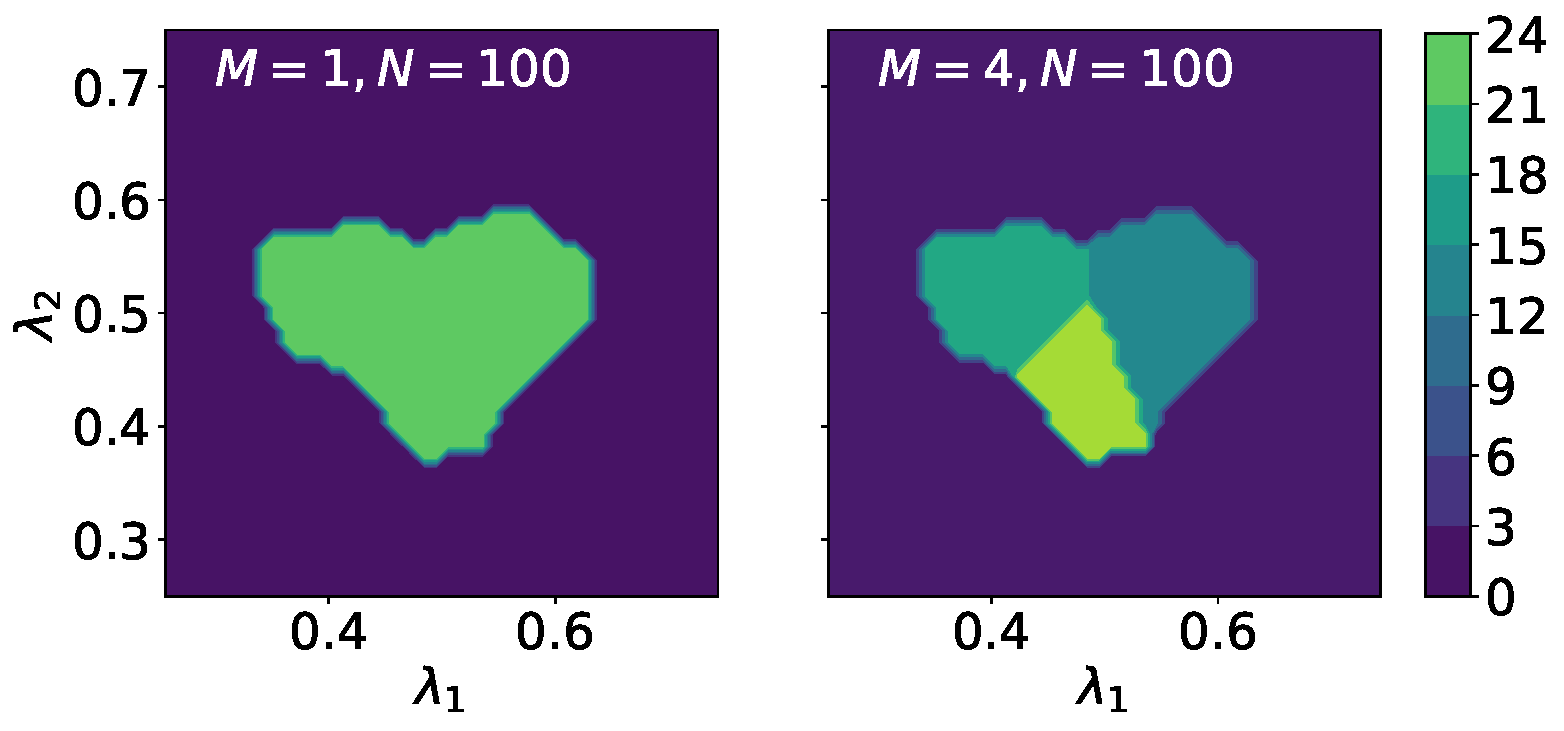
\includegraphics[width=\linewidth]{./examples/identity/set/M1-N100_N100-vs-M4-N100_N100.pdf}
\end{minipage}
\caption{
$\nsamps=100$ were used to discretize $\pspace$ and $\ndiscs=1, 4$ (left/right) were used to discretize $\dspace$.
The latter was chosen to visualize the geometry of describing $\pspace$ with $\pborel$.
}
\label{fig:ex:identity_set_1E2}
\end{figure}

We have chosen a uniform density to describe the uncertainty in our output space.
Any value that is within $0.1$ to the left and right of the reference value \pythoninline{Qref = [0.5, 0.5]} in each dimension is treated as equally likely.
This was done so that using $\ndiscs = 1$ samples to discretize $\dspace$ would fully characterize the characteristic function density representing this uncertainty.
The inverse image of this set is a characteristic function defined on $\pborel$, so errors will exist in particular at the boundaries of the region.

The fundamental challenge with the set-based approach is linked to the geometry of the induced Voronoi-cell tesselation on $\pspace$.
With only $\nsamps = 100$ samples, we see in \ref{fig:ex:identity_set_1E2} that the region (which is supposed to be a square) hardly represents one.
There is ample variation in the shape parameters of the induced sets $\VV_\iparam$ when so few samples are used.
It is possible to ``get lucky'' with the aligning of boundaries between the true target density $\Chi_{[0.4, 0.6]^2}$, but the Figure is representative of the difficulty of using $\nsamps = 100$ random samples to describe a geometry.
With $\nsamps = 1000$, there are usually still significant differences in the symmetric difference of approximated and true supports of the densities.

Below, we demonstrate the use of more samples to resolve the geometry of the desired set.
\begin{figure}[ht]
\begin{minipage}{.975\textwidth}
  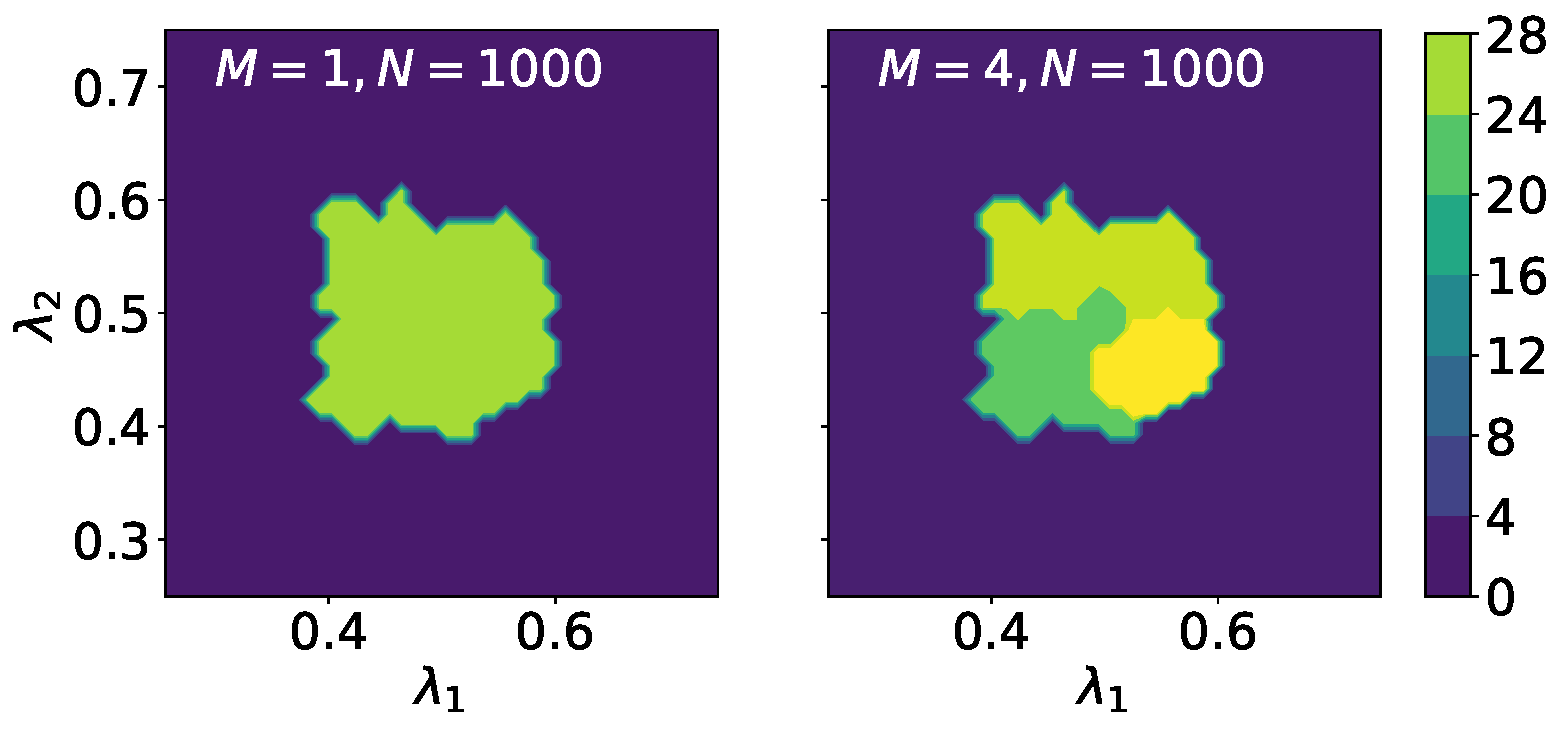
\includegraphics[width=\linewidth]{./examples/identity/set/M1-N1000_N1000-vs-M4-N1000_N1000.pdf}
  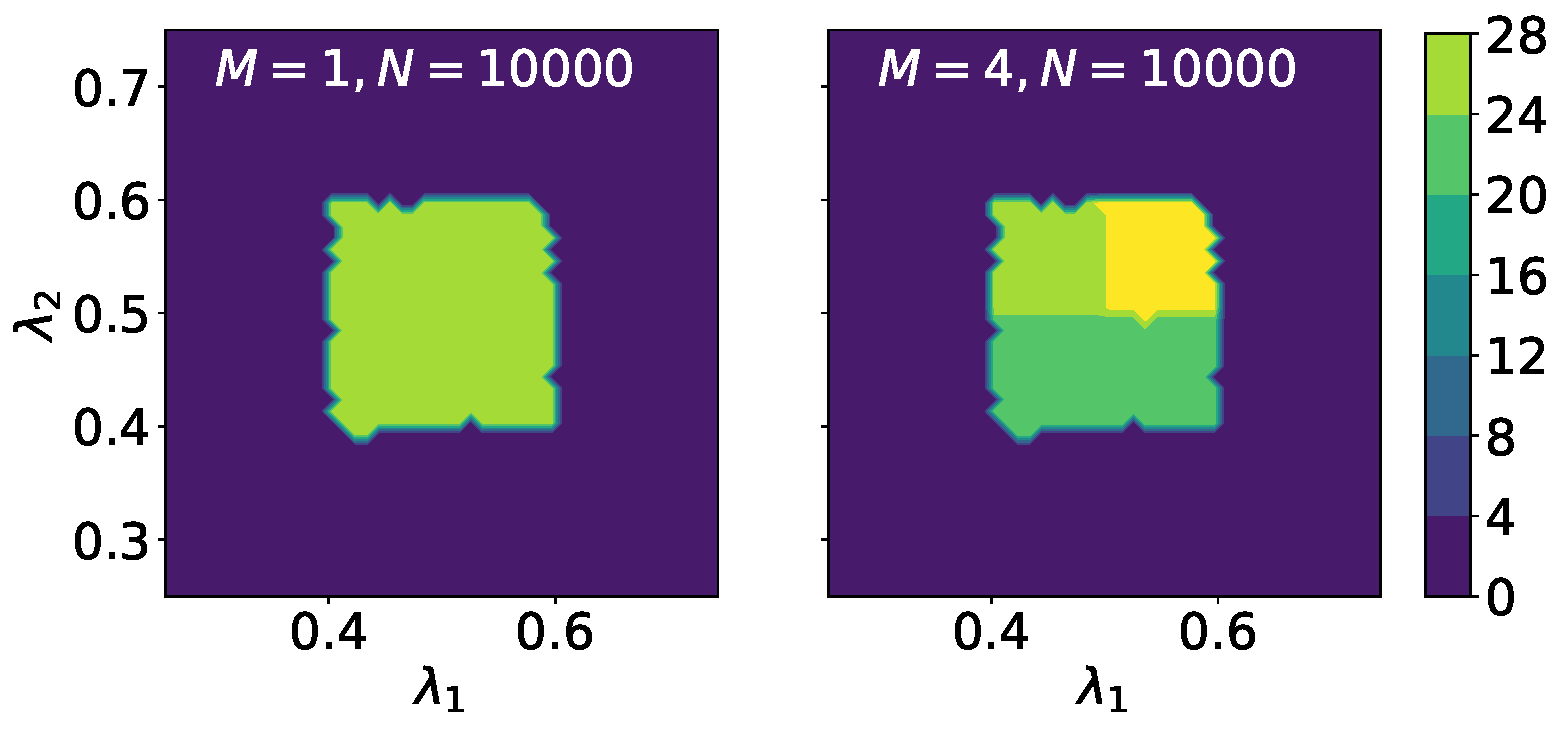
\includegraphics[width=\linewidth]{./examples/identity/set/M1-N10000_N10000-vs-M4-N10000_N10000.pdf}
\end{minipage}
\caption{
(Top):$\nsamps=1,000$ were used to discretize $\pspace$ and $\ndiscs=1, 4$ (left/right) were used to discretize $\dspace$.
(Bottom): The same, except with $\nsamps=10,000$, where we finally begin to see something resembling the correct correct geometry.
}
\label{fig:ex:identity_set_1E3_1E4}
\end{figure}


We remark on the fact that in this particular situation, $\ndiscs = 1$ is a ``correct'' choice for the probability measure chosen, and $\ndiscs = 4$ actually introduces errors.
The reason that the latter solutions have different values inside of the support of $\PPspace$
